\documentclass[12pt]{article}
\usepackage[margin=2cm]{geometry}
\usepackage{amsmath}
\usepackage{graphicx}

\begin{document}

\noindent
The following hydrogen data table is from ``Atomic Transition Probabilities,'' 1966.

\begin{center}
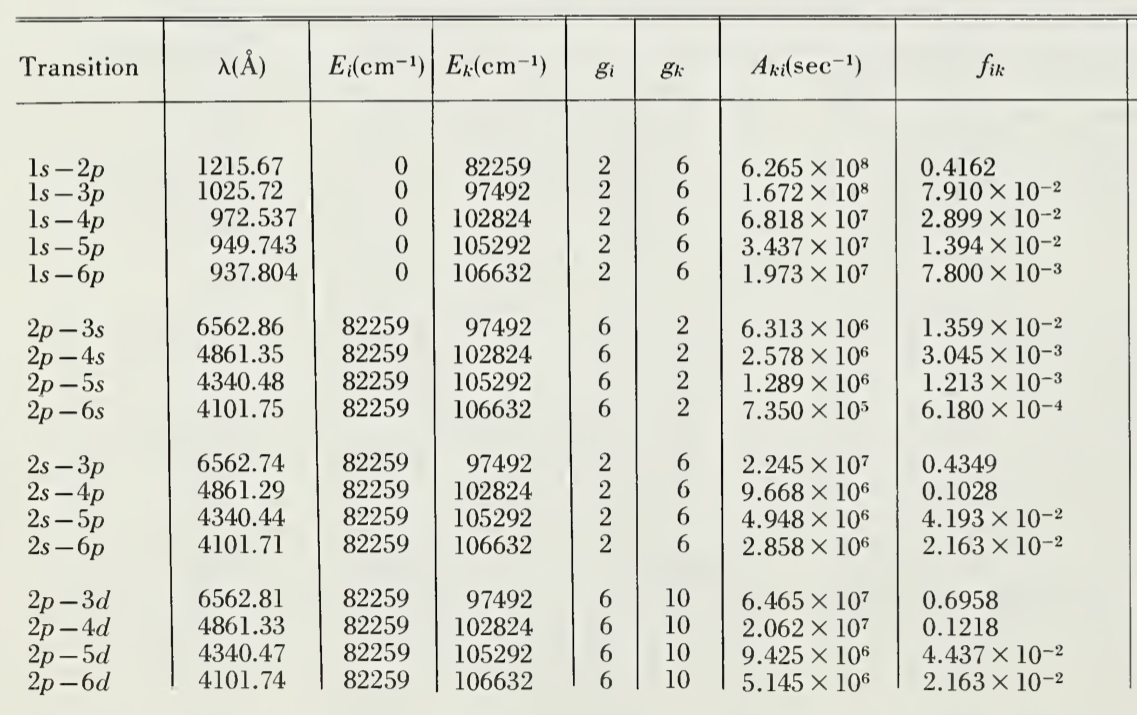
\includegraphics[scale=0.5]{h-alpha-line.png}
\end{center}

\noindent
The $2-3$ transitions correspond to the H-$\alpha$ line of the hydrogen spectrum.
\begin{center}
\begin{tabular}{|c|c|c|}
\hline
Transition & $\lambda$ (\AA) & $A_{ki}$ ($\text{second}^{-1}$)
\\
\hline
$2p-3s$ & 6562.86 & $6.313\times10^6$
\\
$2s-3p$ & 6562.74 & $2.245\times10^7$
\\
$2p-3d$ & 6562.81 & $6.465\times10^7$
\\
\hline
\end{tabular}
\end{center}

\noindent
$A_{ki}$ is the spontaneous emission rate for $k\rightarrow i$.

\bigskip
\noindent
For H-$\alpha$ we have $k=3$ and $i=2$.

\bigskip
\noindent
Let us compute $A_{ki}$ for H-$\alpha$ and see if the results match the table.

\bigskip
\noindent
Orbital names correspond to the following azimuthal quantum numbers.
\begin{center}
\begin{tabular}{|c|c|}
\hline
Name & Azimuthal quantum number $\ell$
\\
\hline
$s$ & $0$
\\
$p$ & $1$
\\
$d$ & $2$
\\
\hline
\end{tabular}
\end{center}

\noindent
Because of the magnetic quantum number $m_\ell$
there are multiple ways for each orbital transition to occur.
($m_\ell=0,\pm1,\ldots,\pm\ell$)

\bigskip
\noindent
There are three transitions for $3s\rightarrow2p$.
\begin{align*}
\psi_{3,0,0}&\rightarrow\psi_{2,1,1}
\\
\psi_{3,0,0}&\rightarrow\psi_{2,1,0}
\\
\psi_{3,0,0}&\rightarrow\psi_{2,1,-1}
\end{align*}

\noindent
There are three transitions for $3p\rightarrow2s$.
\begin{align*}
\psi_{3,1,1}&\rightarrow\psi_{2,0,0}
\\
\psi_{3,1,0}&\rightarrow\psi_{2,0,0}
\\
\psi_{3,1,-1}&\rightarrow\psi_{2,0,0}
\end{align*}

\noindent
Finally, there are fifteen transitions for $3d\rightarrow2p$.
\begin{align*}
\psi_{3,2,2}&\rightarrow\psi_{2,1,1} &
\psi_{3,2,2}&\rightarrow\psi_{2,1,0} &
\psi_{3,2,2}&\rightarrow\psi_{2,1,-1}
\\
\psi_{3,2,1}&\rightarrow\psi_{2,1,1} &
\psi_{3,2,1}&\rightarrow\psi_{2,1,0} &
\psi_{3,2,1}&\rightarrow\psi_{2,1,-1}
\\
\psi_{3,2,0}&\rightarrow\psi_{2,1,1} &
\psi_{3,2,0}&\rightarrow\psi_{2,1,0} &
\psi_{3,2,0}&\rightarrow\psi_{2,1,-1}
\\
\psi_{3,2,-1}&\rightarrow\psi_{2,1,1} &
\psi_{3,2,-1}&\rightarrow\psi_{2,1,0} &
\psi_{3,2,-1}&\rightarrow\psi_{2,1,-1}
\\
\psi_{3,2,-2}&\rightarrow\psi_{2,1,1} &
\psi_{3,2,-2}&\rightarrow\psi_{2,1,0} &
\psi_{3,2,-2}&\rightarrow\psi_{2,1,-1}
\end{align*}

\noindent
For each H-$\alpha$ line, an average $A_{ki}$ is computed by summing over $A_{ki}$ for individual transitions
and dividing by the number of distinct initial states.

\bigskip
\noindent
For example, $3d\rightarrow2p$ has five distinct initial states, so the divisor is five.

\bigskip
\noindent
$A_{ki}$ is computed from the following formula.
\begin{equation*}
A_{ki}=\frac{e^2}{3\pi\varepsilon_0\hbar c^3}\,\omega_{ki}^3\,|r_{ki}|^2
\end{equation*}

\noindent
The transition frequency $\omega_{ki}$ is given by Bohr's frequency condition.
\begin{equation*}
\omega_{ki}=\frac{1}{\hbar}(E_k-E_i)
\end{equation*}

\noindent
The transition probability (multiplied by a physical constant) is
\begin{equation*}
|r_{ki}|^2
=|x_{ki}|^2
+|y_{ki}|^2
+|z_{ki}|^2
\end{equation*}
For wave functions $\psi$ in spherical coordinates we have the following transition amplitudes.
\begin{align*}
x_{ki}&=\int\psi_k^*\,(r\sin\theta\cos\phi)\,\psi_i\,dV
\\
y_{ki}&=\int\psi_k^*\,(r\sin\theta\sin\phi)\,\psi_i\,dV
\\
z_{ki}&=\int\psi_k^*\,(r\cos\theta)\,\psi_i\,dV
\end{align*}

\noindent
Using Eigenmath we obtain the following values for average $A_{ki}$.
\begin{align*}
A_{3s2p}&=6.31358\times10^6\,\text{second}^{-1}
\\
A_{3p2s}&=2.24483\times10^7\,\text{second}^{-1}
\\
A_{3d2p}&=6.4651\times10^7\,\text{second}^{-1}
\end{align*}
These values are essentially identical to the values shown in the table.

\bigskip
\noindent
Some of the $|r_{ki}|^2$ are zero, indicating forbidden transitions.

\bigskip
\noindent
The following tables show $|r_{ki}|^2$ for each transition
(multiply given values by $a_0^2=2.8\times10^{-21}\;\text{meter}^2$).

\bigskip
\noindent
Each row is an initial state $\psi_i$ and each column is a final state $\psi_k$.

\begin{center}
\begin{tabular}{|l|c|c|c|}
\hline
& Final state $\psi_{2,1,1}$ & Final state $\psi_{2,1,0}$ & Final state $\psi_{2,1,-1}$\\
\hline
Initial state $\psi_{3,0,0}$ & 0.293534 & 0.293534 & 0.293534\\
\hline
\end{tabular}
\end{center}

\begin{center}
\begin{tabular}{|l|c|}
\hline
& Final state $\psi_{2,0,0}$\\
\hline
Initial state $\psi_{3,1,1}$ & 3.13103
\\
Initial state $\psi_{3,1,0}$ & 3.13103
\\
Initial state $\psi_{3,1,-1}$ & 3.13103\\
\hline
\end{tabular}
\end{center}

\begin{center}
\begin{tabular}{|l|c|c|c|}
\hline
& Final state $\psi_{2,1,1}$ & Final state $\psi_{2,1,0}$ & Final state $\psi_{2,1,-1}$\\
\hline
Initial state $\psi_{3,2,2}$ & 9.01737 & 0 & 0
\\
Initial state $\psi_{3,2,1}$ & 4.50868 & 4.50868 & 0
\\
Initial state $\psi_{3,2,0}$ & 1.50289 & 6.01158 & 1.50289
\\
Initial state $\psi_{3,2,-1}$ & 0 & 4.50868 & 4.50868
\\
Initial state $\psi_{3,2,-2}$ & 0 & 0 & 9.01737\\
\hline
\end{tabular}
\end{center}

\end{document}
